\section{提案手法}

\subsection{全体構成}
提案システムは，(1) 入力文または読みを母音列へ変換する母音化部，
(2) 母音列（と任意の文脈）から日本語候補を生成・順位付けする LLM 候補生成部，
からなる（図\ref{fig:overview}）．
ユーザは 5 母音と撥音のみを入力し，システムが上位 $k$ 件の候補文を提示する．

\begin{figure}[t]
  \centering
  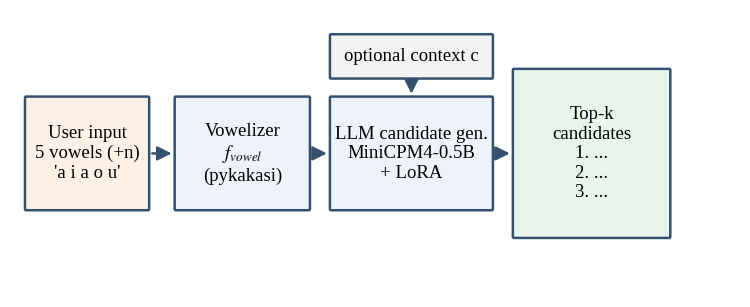
\includegraphics[width=0.95\columnwidth]{figures/fig_overview.png}
  \caption{提案システムの概要．母音列（＋任意の文脈）から上位$k$候補を生成・提示する．}
  \label{fig:overview}
\end{figure}

\subsection{母音化}
入力文または読み列を $x$，母音列を $\bm{v}$ とし，母音化を写像 $f_{\mathrm{vowel}}$ で表す．
\begin{equation}
  \bm{v} = f_{\mathrm{vowel}}(x)
\end{equation}
実装では，漢字を含む任意文を pykakasi により読み（ひらがな）へ変換し，
各かなを 1 母音記号へ写像して空白区切りで出力する．
コードから確認した写像規則は表\ref{tab:vowelrule}の通りである．

\begin{table}[t]
  \centering\small
  \caption{母音化規則}
  \label{tab:vowelrule}
  \begin{tabular}{ll}
    \toprule
    対象 & 扱い \\
    \midrule
    清音・濁音・半濁音 & 母音 \texttt{a/i/u/e/o} に写像 \\
    撥音「ん」 & \texttt{n} \\
    拗音「ゃゅょ」 & 2 文字を 1 母音に集約（例 きょ$\to$\texttt{o}）\\
    促音「っ」 & 無視（出力しない）\\
    長音「ー」 & 無視（例 コーヒー$\to$\texttt{o i}）\\
    小書き「ゎゕゖ」 & 無視 \\
    カタカナ & 一旦ひらがな化して母音化 \\
    句読点・記号 & 出力に現れない \\
    数字・英字 & 読みが付かず脱落（例 100$\to$空，ABC$\to$空）\\
    \bottomrule
  \end{tabular}
\end{table}

この写像により，「今日は天気が悪かった」は
\texttt{o n i i a e n i a a u a a} となる．
子音・濁清の区別が失われるため，同一母音列に複数の日本語表現が対応する
本質的曖昧性が生じる（「寒い」「暑い」$\to$\texttt{a u i}）．

\subsection{候補生成と順位付け}
母音列 $\bm{v}$ から日本語文 $y$ を生成する条件付き分布 $P_\theta(y\mid \bm{v})$ を LLM で表す．
最尤候補は
\begin{equation}
  \hat{y} = \arg\max_{y} P_\theta(y \mid \bm{v})
\end{equation}
であり，上位 $k$ 件の候補集合を
\begin{equation}
  \mathcal{Y}_k(\bm{v}) = \operatorname*{TopK}_{y} P_\theta(y \mid \bm{v})
\end{equation}
と定義する．実装ではビーム探索（ビーム幅 8）により $\mathcal{Y}_k$ を生成し，
重複を除いた上位 $k$ 件を候補として提示する．
任意で直前の文を文脈 $c$ として与えられ，その場合は $P_\theta(y\mid \bm{v}, c)$ を用いる．

\subsection{LoRA による追加学習}
候補生成器は事前学習済み LLM を LoRA で追加学習して得る．
事前学習済み重みを $W$，学習対象の低ランク行列を $A, B$，rank を $r$，スケーリング係数を $\alpha$ とすると，
\begin{equation}
  W' = W + \Delta W = W + BA
\end{equation}
\begin{equation}
  h = Wx + \frac{\alpha}{r}BAx
\end{equation}
であり，$W$ を固定して $A, B$ のみを学習する．
これにより全パラメータ更新に比べ少ない学習量でタスク適応が可能となる．
本研究では母音列$\to$文の生成を教師あり微調整（SFT）として学習し，
損失はプロンプト部をマスクして文（と EOS）部にのみ与える．
